\documentclass[border=8pt]{standalone}

% --- packages (mirror these in figure.meta.json "requires") ---
\usepackage{tikz}
\usepackage{amsmath}
\usetikzlibrary{positioning, arrows.meta}

% --- palette (canonical source: skills/color-palettes/skill.md; light variant) ---
\definecolor{otblue}{HTML}{0072B2}
\definecolor{otorange}{HTML}{E69F00}
\definecolor{otteal}{HTML}{009E73}
\definecolor{otpurple}{HTML}{CC79A7}
\definecolor{otgray}{HTML}{5A5A5A}

\begin{document}
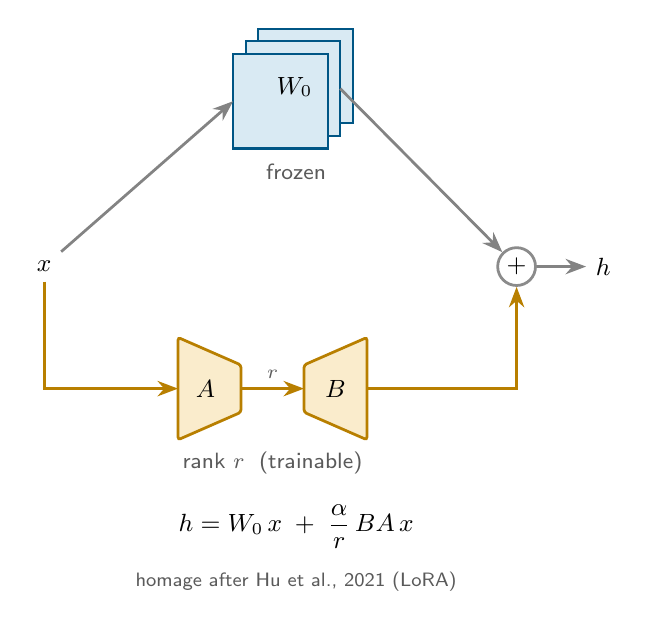
\begin{tikzpicture}[
    >={Stealth[length=2.6mm]},
    font=\sffamily,
    flow/.style={draw=otgray!75, line width=1pt, ->},
    lowrank/.style={draw=otorange!80!black, line width=1pt, ->},
    note/.style={font=\sffamily\small, text=otgray},
  ]
  % ----- input -----
  \node[font=\small] (x) at (0,0) {$x$};

  % ----- frozen pretrained weights W0: a stacked slab (the 'layer' motif), blue -----
  \begin{scope}[shift={(2.4,1.5)}]
    \foreach \i in {2,1,0}{
      \pgfmathsetmacro{\d}{\i*0.16}
      \filldraw[draw=otblue!75!black, fill=otblue!15, line width=0.8pt]
        (\d,\d) rectangle (\d+1.2,\d+1.2);
    }
    \node[font=\small] at (0.78,0.78) {$W_0$};
    \coordinate (Wc) at (0.78,0.78);
    \coordinate (Win) at (0,0.6);
    \coordinate (Wout) at (1.36,0.76);
  \end{scope}
  \node[note, font=\sffamily\footnotesize] at (3.2,1.2) {frozen};

  % ----- low-rank update B A : an encoder->decoder bottleneck, orange -----
  % A: down-projection d -> r  (wide -> narrow)
  \filldraw[draw=otorange!80!black, fill=otorange!20, line width=1pt, rounded corners=1pt]
    (1.7,-2.2) -- (1.7,-0.9) -- (2.5,-1.25) -- (2.5,-1.85) -- cycle;
  \node[font=\small] at (2.05,-1.55) {$A$};
  % B: up-projection r -> d  (narrow -> wide)
  \filldraw[draw=otorange!80!black, fill=otorange!20, line width=1pt, rounded corners=1pt]
    (3.3,-1.25) -- (3.3,-1.85) -- (4.1,-2.2) -- (4.1,-0.9) -- cycle;
  \node[font=\small] at (3.7,-1.55) {$B$};
  \node[note, font=\sffamily\footnotesize] at (2.9,-2.5) {rank $r$ \;(trainable)};

  % ----- sum and output -----
  \node[draw=otgray!70, line width=1pt, circle, inner sep=1.5pt, font=\small] (sum) at (6.0,0) {$+$};
  \node[font=\small] (h) at (7.1,0) {$h$};

  % ----- wiring -----
  \draw[flow] (x) -- (Win);                       % x -> W0
  \draw[flow] (Wout) -- (sum);                    % W0 x -> +
  \draw[lowrank] (x) |- (1.7,-1.55);              % x -> A
  \draw[lowrank] (2.5,-1.55) -- (3.3,-1.55) node[midway, above, note, font=\sffamily\scriptsize] {$r$};
  \draw[lowrank] (4.1,-1.55) -| (sum);            % B A x -> +
  \draw[flow] (sum) -- (h);

  % ----- equation + provenance -----
  \node[font=\small] at (3.2,-3.3) {$h = W_0\,x \;+\; \dfrac{\alpha}{r}\,B A\,x$};
  \node[note, font=\sffamily\scriptsize] at (3.2,-4.0) {homage after Hu et al., 2021 (LoRA)};

\end{tikzpicture}
\end{document}
